% !TEX root = ../MasterThesis_Onoe.tex
% 上記はただのコメントではなく親ファイルの場所を教えているので
% 消してしまうとファイルごとのタイプセットができなくなるので注意。
% 親ファイル名を変更したときはここも変更する。

\chapter{序論} \label{sec:Intruduction}
本章では、はじめに1.1節で素粒子とそれらに働く相互作用を説明する標準模型(The Standard Model, SM)について述べる。そして1.2節にて将来の電子陽電子ヒッグスファクトリーである、国際リニアコライダー計画(International Linear Collider, ILC)の概要に触れたのち、1.3節でILCが探索する物理、1.4節でILCのについて述べる。
\section{素粒子標準理論}
素粒子とは、物質を構成している究極要素をさす名称である。そして素粒子物理学は、それら構成要素とその間に働く相互作用の性質を解明する学問である。現代の素粒子物理学では、すべての現象を説明するための基本的な枠組みとして図\ref{sm}のような標準模型を掲げており、これは現時点の実験データと高い精度で一致することが確認されている。\\
\begin{figure}[ht]
	\begin{center}
 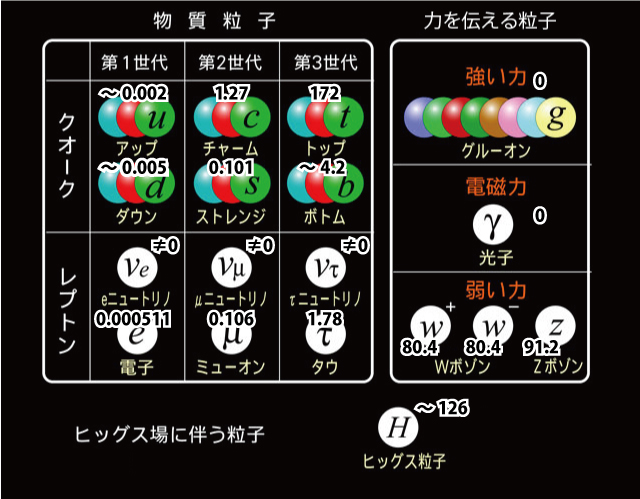
\includegraphics[keepaspectratio, scale=0.4]
 	{Figure/Introduction/sm.jpg}
 		\caption{素粒子の標準模型(数値は質量[$GeV/c^2$])}
 		\label{sm}
	\end{center}
\end{figure}
 標準理論は、主に次に挙げる2つの公理に沿って記述されている。1つ目に、物質の究極要素である素粒子はクォークとレプトンというスピン1/2のフェルミオンである。2つ目に、素粒子の相互作用はゲージ粒子によって記述され、標準理論における相互作用は電磁相互作用・弱い相互作用・強い相互作用の3つである。\\
 物質の化学的性質を失わない最小単位は分子であり、分子はさらに原子の組み合わせによって構成されている。そして原子は原子核と電子によって構成されており、原子核は陽子と中性子のような核子からなっている。この核子を構成するものがクォークであり、標準模型においては6種類存在する。また同様に素粒子であり、核力のような強い相互作用をしないものをレプトンと呼び、同様に6種類存在する。クォーク・レプトンともに3つの世代と2つの電荷タイプをもっており、世代の高い粒子ほど重いため弱い相互作用により低い世代のクォークへと崩壊する。\\
 素粒子の相互作用を媒介するスピン1のゲージ粒子には、グルーオン・光子・Wボソン・Zボソンの4種類がある。クォークとグルーオンの相互作用である強い相互作用は、量子色力学に基づき$SU(3)$対称性をもつ。また、荷電粒子と光子の相互作用である電磁相互作用とW・Zボソンを介する弱い相互作用は統一され電弱相互作用と呼ばれており、$SU(2)\times U(1)$対称性をもつ。これに加えて重力相互作用が存在するが、他の3つの相互作用と比較して非常に弱く、標準模型では扱われない。\\
 これらゲージ粒子はゲージ対称性を持っており質量は0である必要があるが、先述のW・Zボソンはそれぞれ$80.4\ GeV/c^2$、$91.2\ GeV/c^2$の質量を持っている。標準理論ではこれを説明するためにヒッグス機構を導入し、ゲージ対称性が自発的に破れることで質量を獲得している。このヒッグス機構では真空にスカラー場を導入しており、これとゲージ場との相互作用によって質量を持つことになるが、同時に場に対応する粒子としてヒッグス粒子の存在が必要となる。このヒッグス粒子は2012年7月に欧州原子核研究機構(CERN)の大型ハドロン衝突型加速器(LHC)におけるATLAS、CMS実験によって発見され、理論と実験との一致が確認された。本論文のテーマであるヒッグスファクトリーは、このヒッグス粒子を大量に生成することで、ヒッグス粒子の詳細な研究を目的としている。\\
\section{国際リニアコライダー計画: ILC}
国際リニアコライダー(InternationalLinearCollider:ILC)は、岩手県北上山地に建設が計画されている電子陽電子衝突型線形加速器である。(図\ref{ilc})全長20kmの線形加速器を用いて電子と陽電子を加速し、中央のInteraction Point(IP)で衝突させることで様々な粒子を生成し、これを解析することでヒッグス粒子を始めとする新物理を探索することを目的としている。またILCは重心系エネルギー$\sqrt{s} = 250$\ GeVでの運転開始を予定しているが、線形加速部を延長することで最大1\ TeVまでのアップグレードも可能になっている。\\
\begin{figure}[t]
	\begin{center}
 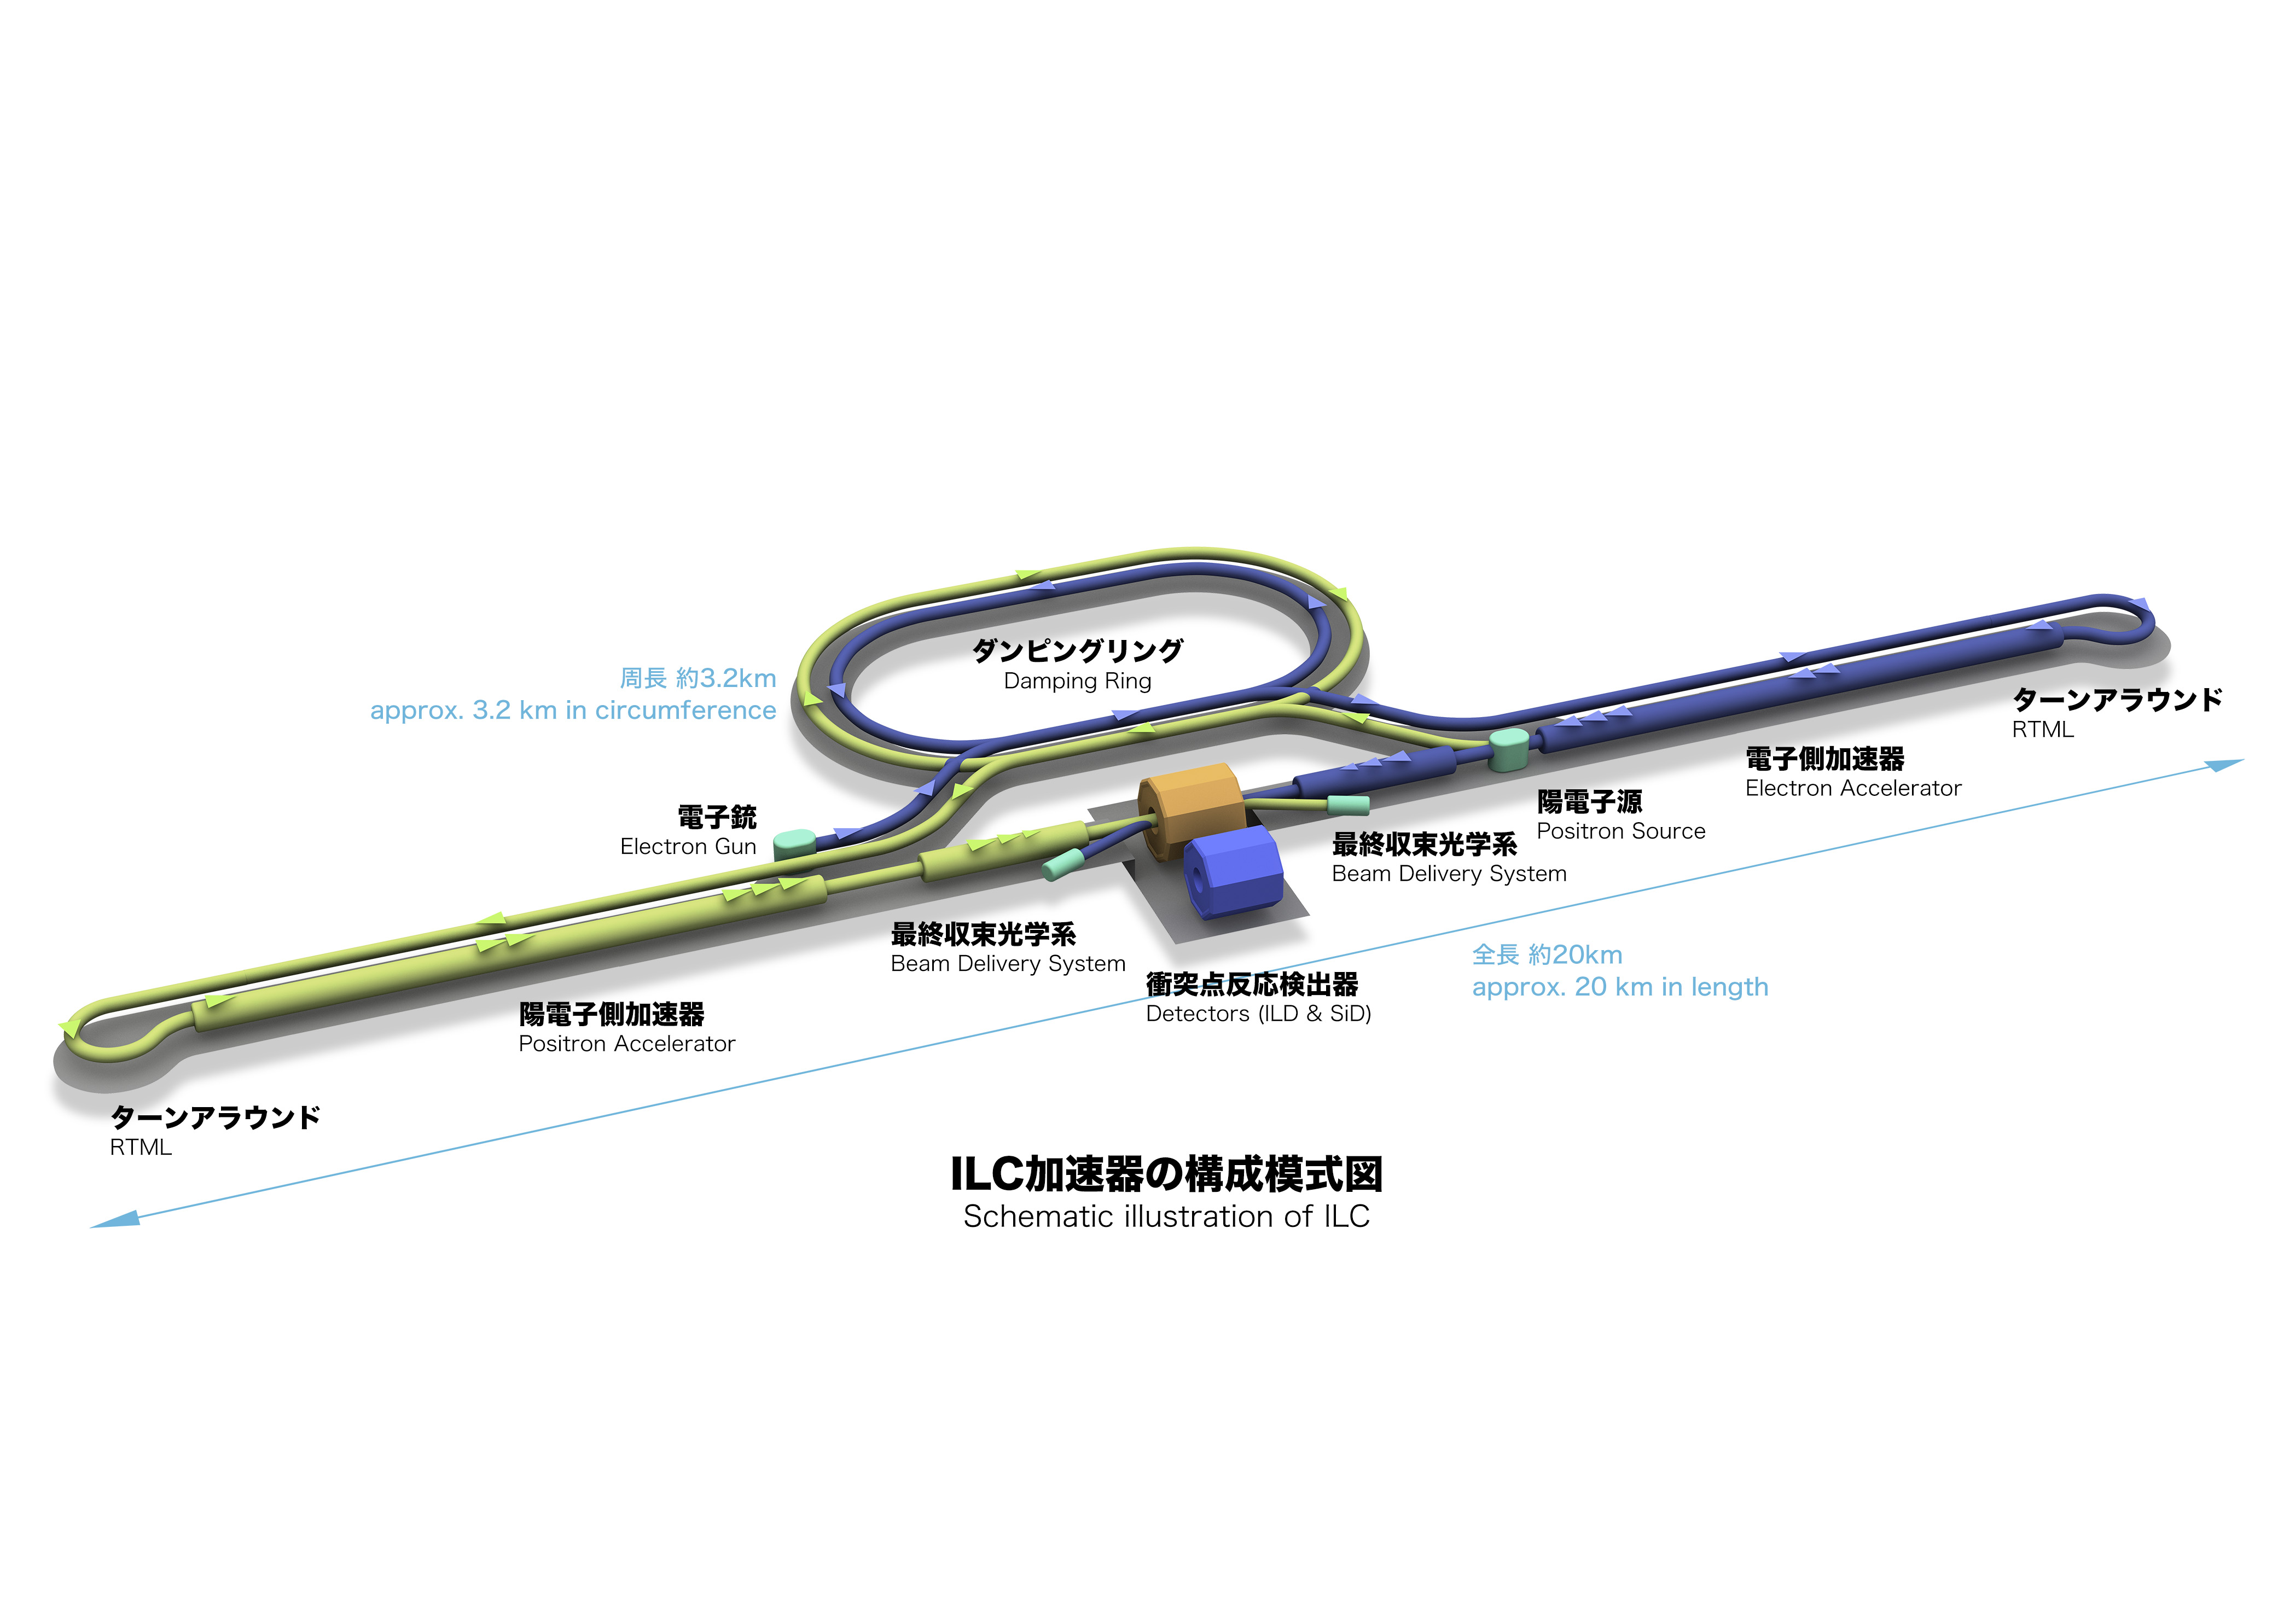
\includegraphics[keepaspectratio, scale=0.3]
 	{Figure/Introduction/ilc.jpg}
 		\caption{ILCの概略図}
 		\label{ilc}
	\end{center}
\end{figure}
 ヒッグス粒子を発見したLHCと比較してILCには以下の2つの利点が存在する。1つ目はLHCが複合粒子であるハドロンのコライダーであるのに対して、ILCはレプトンコライダーである点である。ILCでは背景事象が少ないクリーンな環境で、ヒッグス粒子を始めとした網羅的な新物理探索が可能になっている。また、LHCでは断面積を計算する上でQCDに基づく系統的な不確定性が存在するが、ILCでは電弱相互作用のみについて考えることができるため、高精度な理論検証が可能になる。2つ目は加速粒子である電子陽電子が粒子反粒子の関係にある点である。粒子反粒子が対消滅することで全エネルギーを目的粒子の生成に効率的に用いることができる。加えて全事象を記録しオフラインで事象選択を行うことができるため、トリガーレスで運転することが可能である。
\section{ILCの物理}
\subsection{ヒッグス粒子の精密測定}
1.1節で述べた通り、ILCはヒッグスファクトリーとしての役割を期待されている。ヒッグスファクトリーでは、ヒッグス粒子と大量に生成し崩壊過程を精密測定することで、他の粒子との結合定数を測定し標準模型を検証することができる。ILCにおけるヒッグス粒子の生成断面積は図\ref{higgs_cs}のようになっており、運転開始で予定している$\sqrt{s}=250\ GeV$付近では、主にZH随伴生成過程の断面積が最大となる。このZH随伴生成過程では、反跳粒子であるZボソンを正確に測定することでヒッグス粒子の質量を高い精度で再構成することができる。\\
\begin{figure}[h]
 \begin{minipage}[h]{.45\linewidth}
 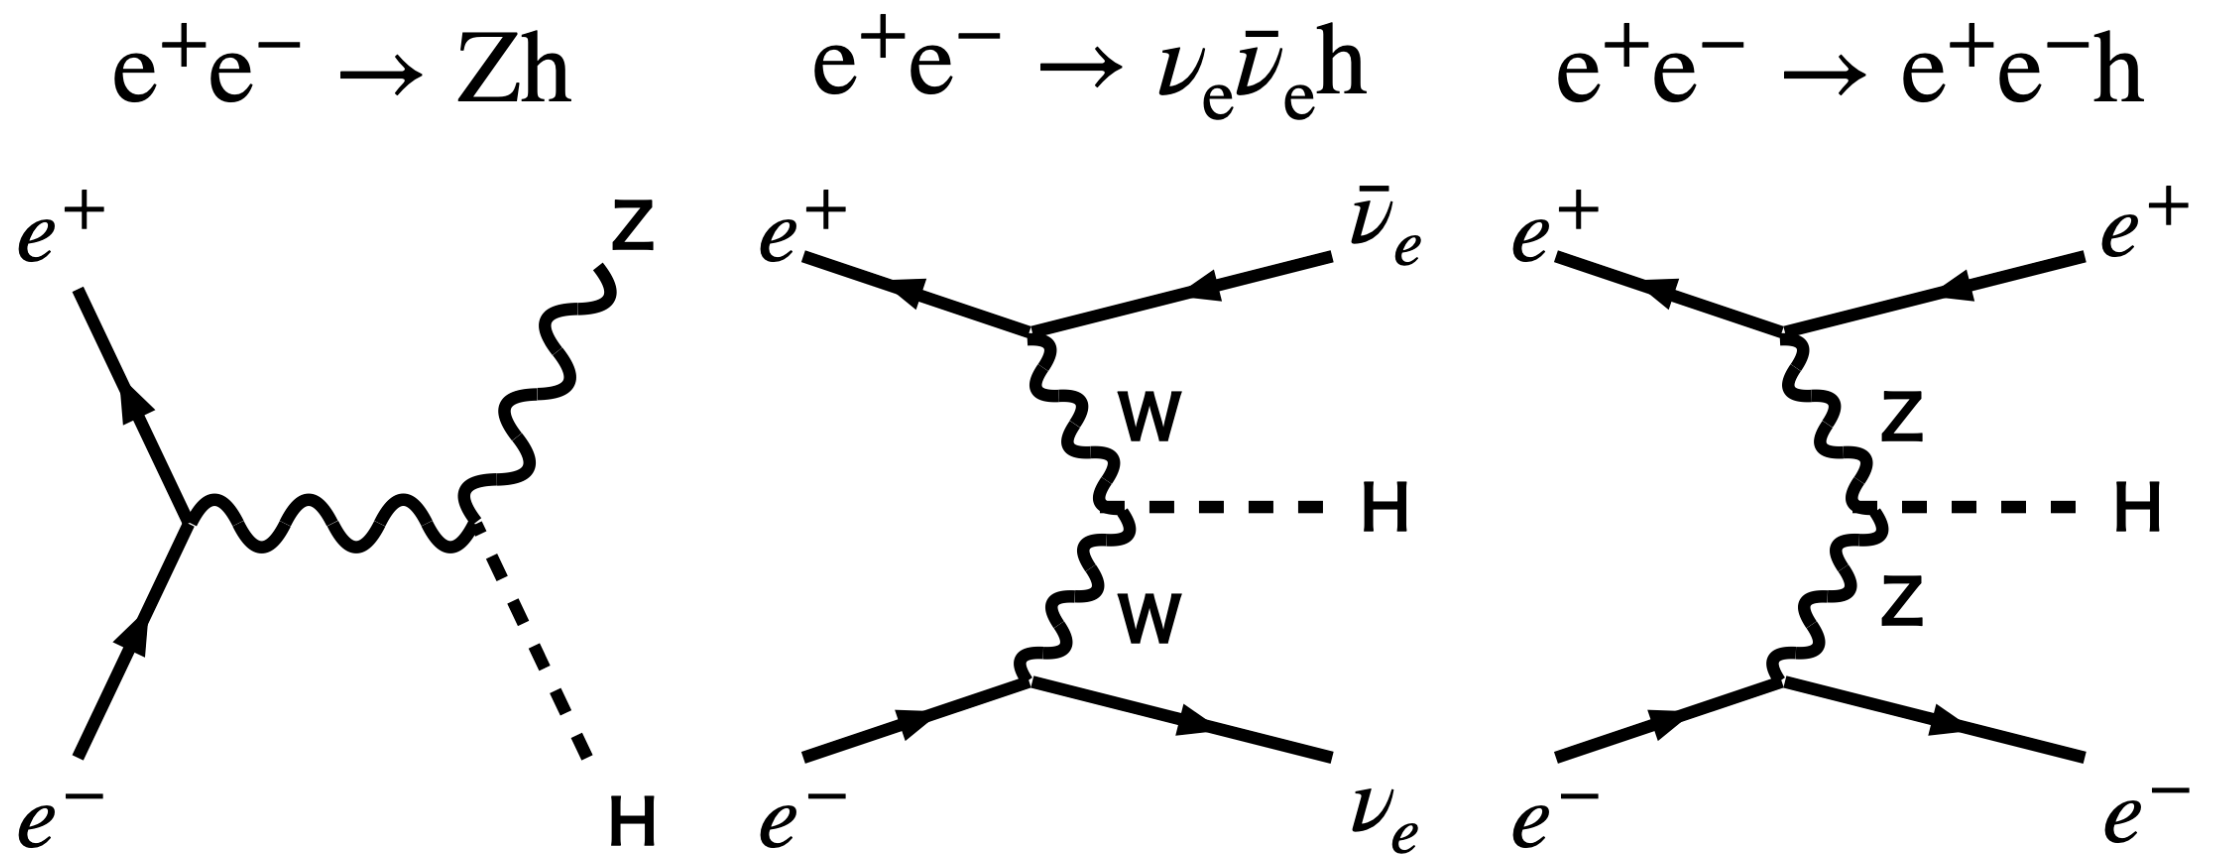
\includegraphics[keepaspectratio, scale=0.18]
 	{Figure/Introduction/higgs_cs_feynman.png}
\end{minipage}
\hfill
 \begin{minipage}[h]{.45\linewidth}
 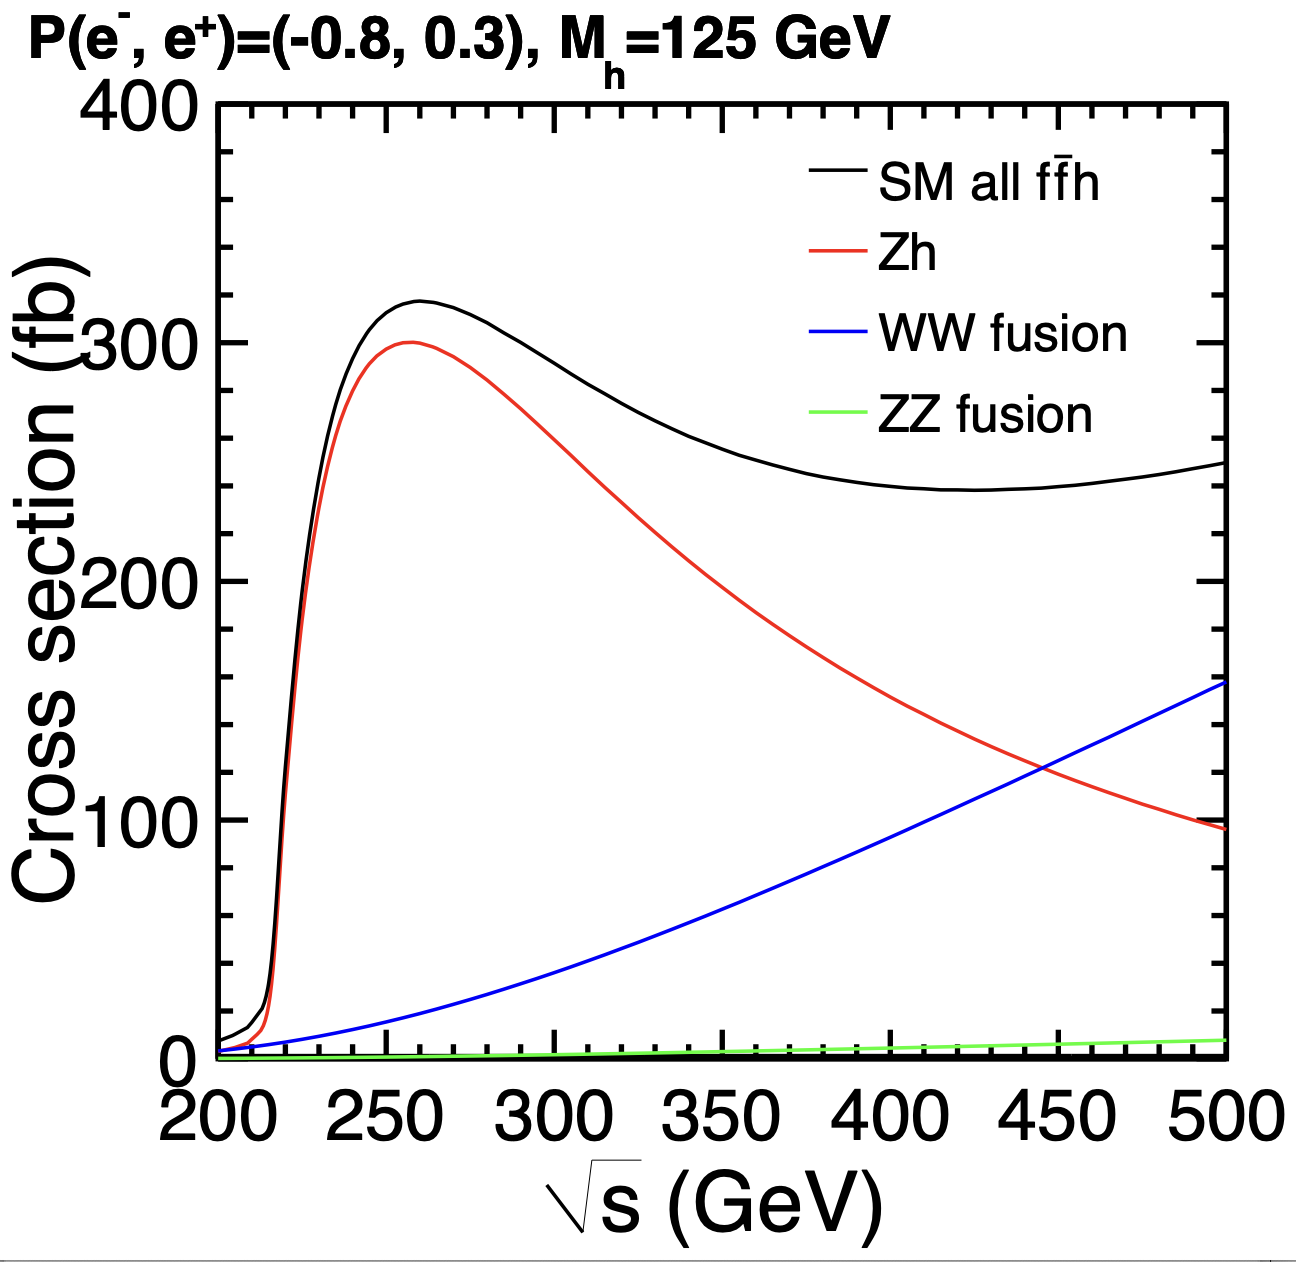
\includegraphics[keepaspectratio, scale=0.25]
 	{Figure/Introduction/higgs_cross_section.png}
\end{minipage}
\label{higgs_cs}
\caption{(左)ILCにおけるヒッグス生成断面積。ヒッグス粒子の質量が$m_h=125$\ GeVであるとして、ZH随伴生成、WW fusion、ZZ fusionをそれぞれ赤、青、緑線で示している。またこのとき電子・陽電子の偏極は、それぞれ電子が左巻き90\%、右巻き10\%の80\%であり、陽電子は左巻き35\%、右巻き65\%の30\%としている。(右)ZH随伴生成、WW fusion、ZZ fusionにおけるファインマンダイアグラム。}
\end{figure}
また電子陽電子衝突によって生成されるヒッグス粒子は不安定であるため、質量の小さい2つの粒子に崩壊する。標準理論におけるヒッグス粒子の崩壊分岐比は図\ref{higgs_decay}のようになっており、ILC250\ GeVにおける崩壊分岐比は表\ref{HiggsDecayonILC}のようになっている。この分岐比の測定精度は信号事象をS、背景事象をNとするとS/$\sqrt{S+N}$となり、背景事象の影響を十分低減させることができた場合には不定性を1\%以下まで下げることができる。そのため、高い検出器性能と精度の高い事象再構成・解析手法が求められる。\\
\begin{figure}[H]
 \begin{minipage}[h]{.45\linewidth}
	\begin{center}
 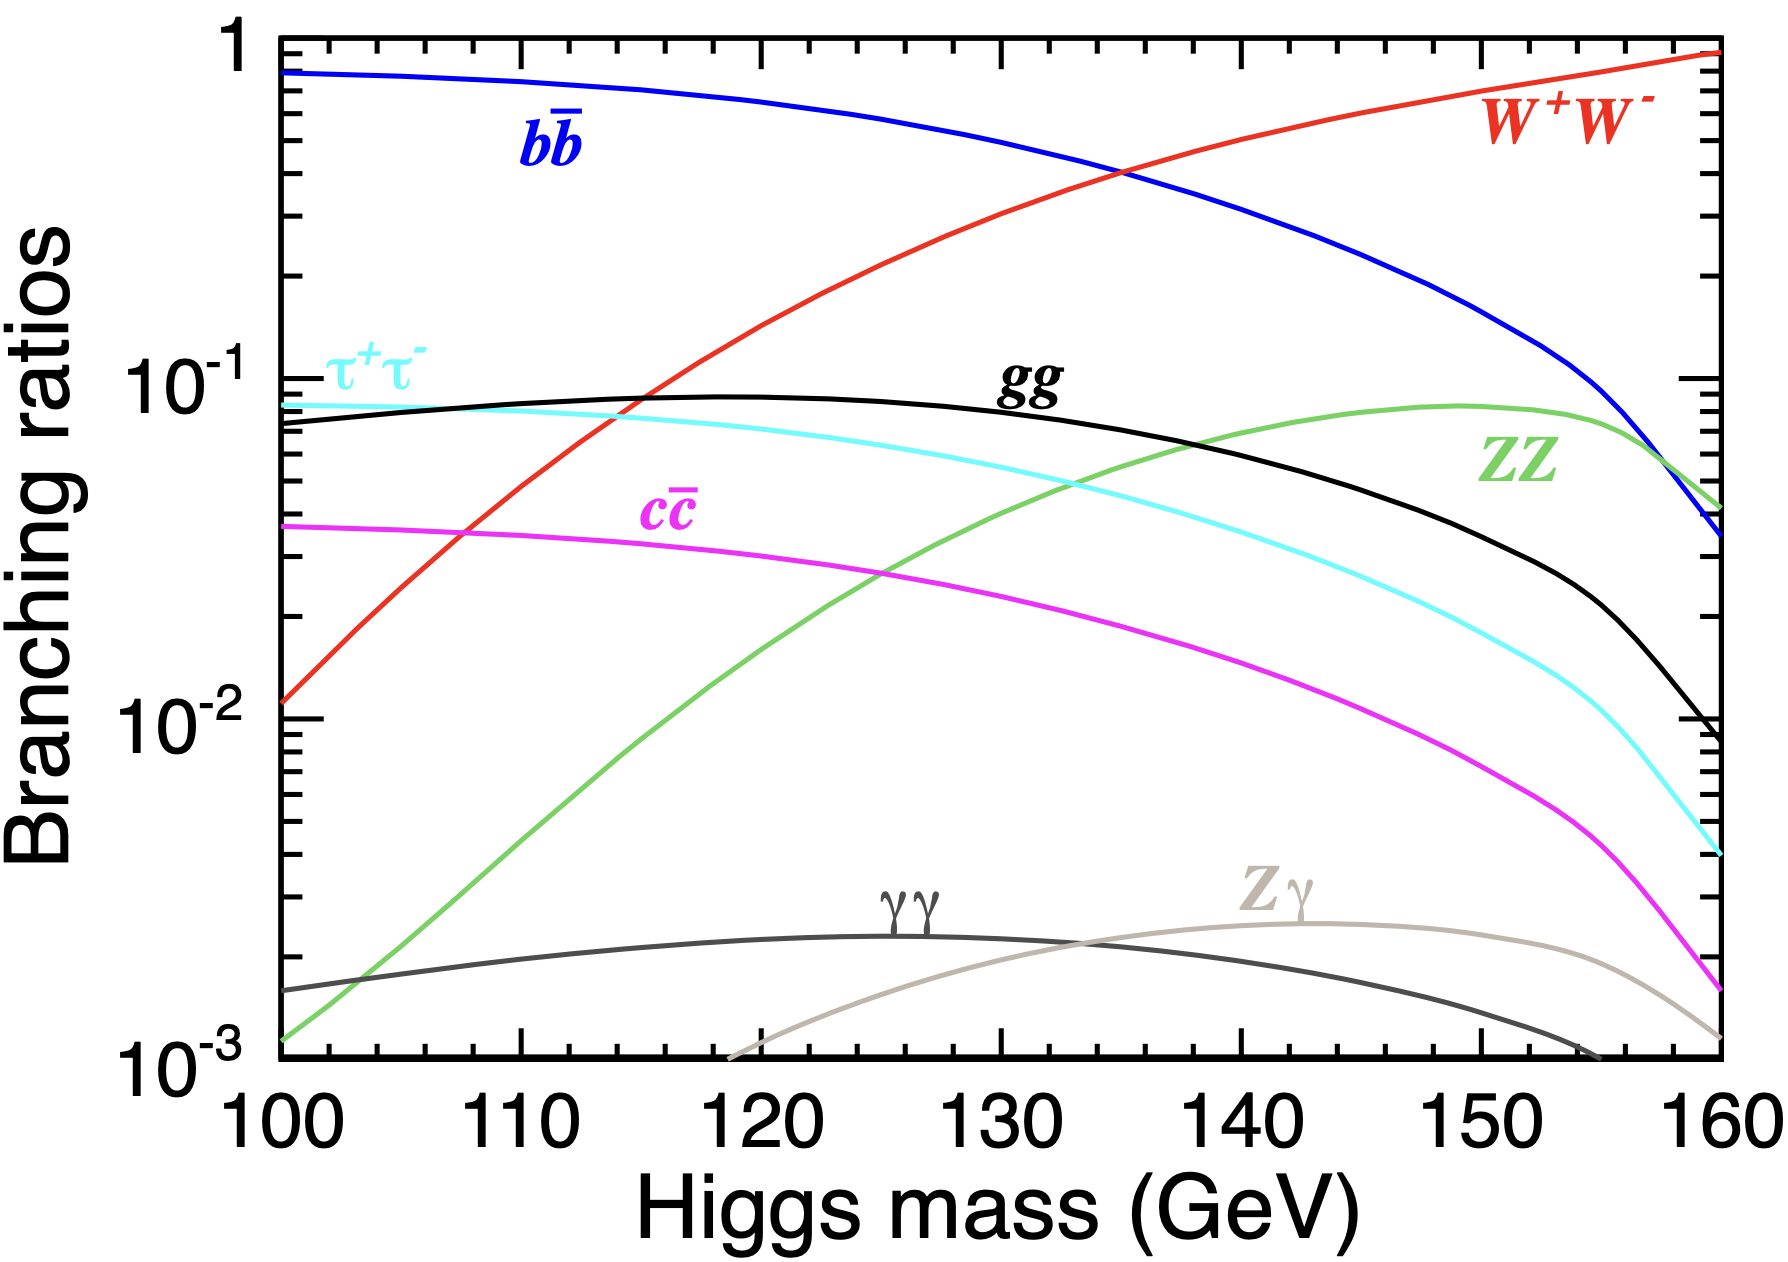
\includegraphics[keepaspectratio, scale=0.2]
 	{Figure/Introduction/higgs_decay.png}
 		\caption{標準理論におけるヒッグス粒子の質量と崩壊分岐比の関係}
 		\label{higgs_decay}
	\end{center}
 \end{minipage}
 \hfill
% ----- 表: ヒッグス崩壊分岐比 ------
\begin{minipage}[h]{.45\linewidth}
\def\@captype{table}
 \centering
  \begin{tabular}{clll}
   \hline
   崩壊モード & 崩壊分岐比\\
   \hline \hline
   $b\bar{b}$ & 58.1\%\\
   $WW$ & 21.5\%\\
   $gg$ & 8.2\%\\
   ${\tau}^+ {\tau}^-$ & 6.3\%\\
   $c \bar{c}$ & 2.9\%\\
   $ZZ$ & 2.6\%\\
   $\gamma \gamma$ & 0.2\%\\
   \hline
  \end{tabular}
   \caption{ILC250GeVにおけるSMヒッグス粒子の崩壊分岐比}
   \label{HiggsDecayonILC}
 \end{minipage}
 \end{figure}
% --------------------
\subsection{階層性問題}
ヒッグス粒子の質量はLHCによって$125\ GeV/c^2$と測定されている。しかしヒッグス粒子の質量は、繰り込みにおいて図\ref{hierarchy}のような高次ダイアグラムから質量補正を受けることで発散してしまい、プランクスケール程度の質量を持ってしまうことが分かっている。そのため標準模型を超える新物理(BSM)がないと仮定すると、質量の量子補正をキャンセルする解決策がなければ$125GeV/c^2$程度の質量を理論的に再現することができない。(ファインチューニング)これを回避するために、以下に挙げるようなTeVスケールの超対称性理論や余剰次元理論など新物理によるシナリオが提案されている。これらシナリオにおけるヒッグス粒子との結合定数は標準理論における予測からズレることとなるため、ILCにおいてヒッグス粒子の精密測定を行うことの意義は大きい。
\begin{figure}[h]
	\begin{center}
 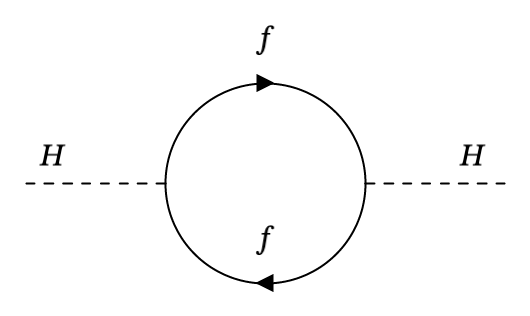
\includegraphics[keepaspectratio, scale=0.4]
 	{Figure/Introduction/feynman.png}
 		\caption{ヒッグス粒子の質量補正となるフェルミオンループ}
 		\label{hierarchy}
	\end{center}
\end{figure}
\subsubsection{超対称性理論}
超対称性理論(Supersymmetry, SUSY)は、フェルミオンとボソンを交換する変換に対する不変性(超対称性)を定義する理論である。またこの理論においては、標準模型におけるすべての粒子に対してスピンが1/2異なる超対称性パートナーが導入される。超対称性が完全である場合、標準模型粒子と質量や相互作用が同じである必要性があるが、現段階ではSUSY粒子は発見に至っていない。しかし階層性問題においては、超対称性によりヒッグスボソンの質量補正に関する2次の発散をフェルミオンの寄与で打ち消し、対数による発散に落とすことができる。
\subsubsection{余剰次元理論}
余剰次元理論とは、四次元時空以外にも次元があるとする理論である。この理論では時空間の次元数を増やすことで、増えた次元のゲージ場にヒッグス場の起源を求める。この場合にはゲージ不変性により、繰り込みの発散が現れないため階層性問題に対応できる。
\subsection{その他の新物理}
上にあげた階層性問題に関する物理に加え、WIMP (Weakly Interacting Massive Particle)など暗黒物質に関する未解決問題に対して探索が可能である。さらに、重心系エネルギー350GeV以上ではトップクォークの質量を精密測定や電弱相互作用の精密検証が可能であり、ILCの実現やそのアップグレードを通して宇宙の謎に迫る大発見を期待することができる。
\section{ILCの検出器}
ILC の検出器(図\ref{detector})には、日本の国々が中心となって開発が進められている International Large Detector(ILD)と、米国が中心となって開発が進められている Silicon Detector (SiD) の二つのコンセプトが提案されており、ILC ではこれら2つの検出器がIPを共有できるように push-pulll 方式を採用している。またILD、SiDともに後述のParicle Flow Algorithm(PFA)という事象再構成アルゴリズムに沿って最適化されている。
\begin{figure}[h]
	\begin{center}
 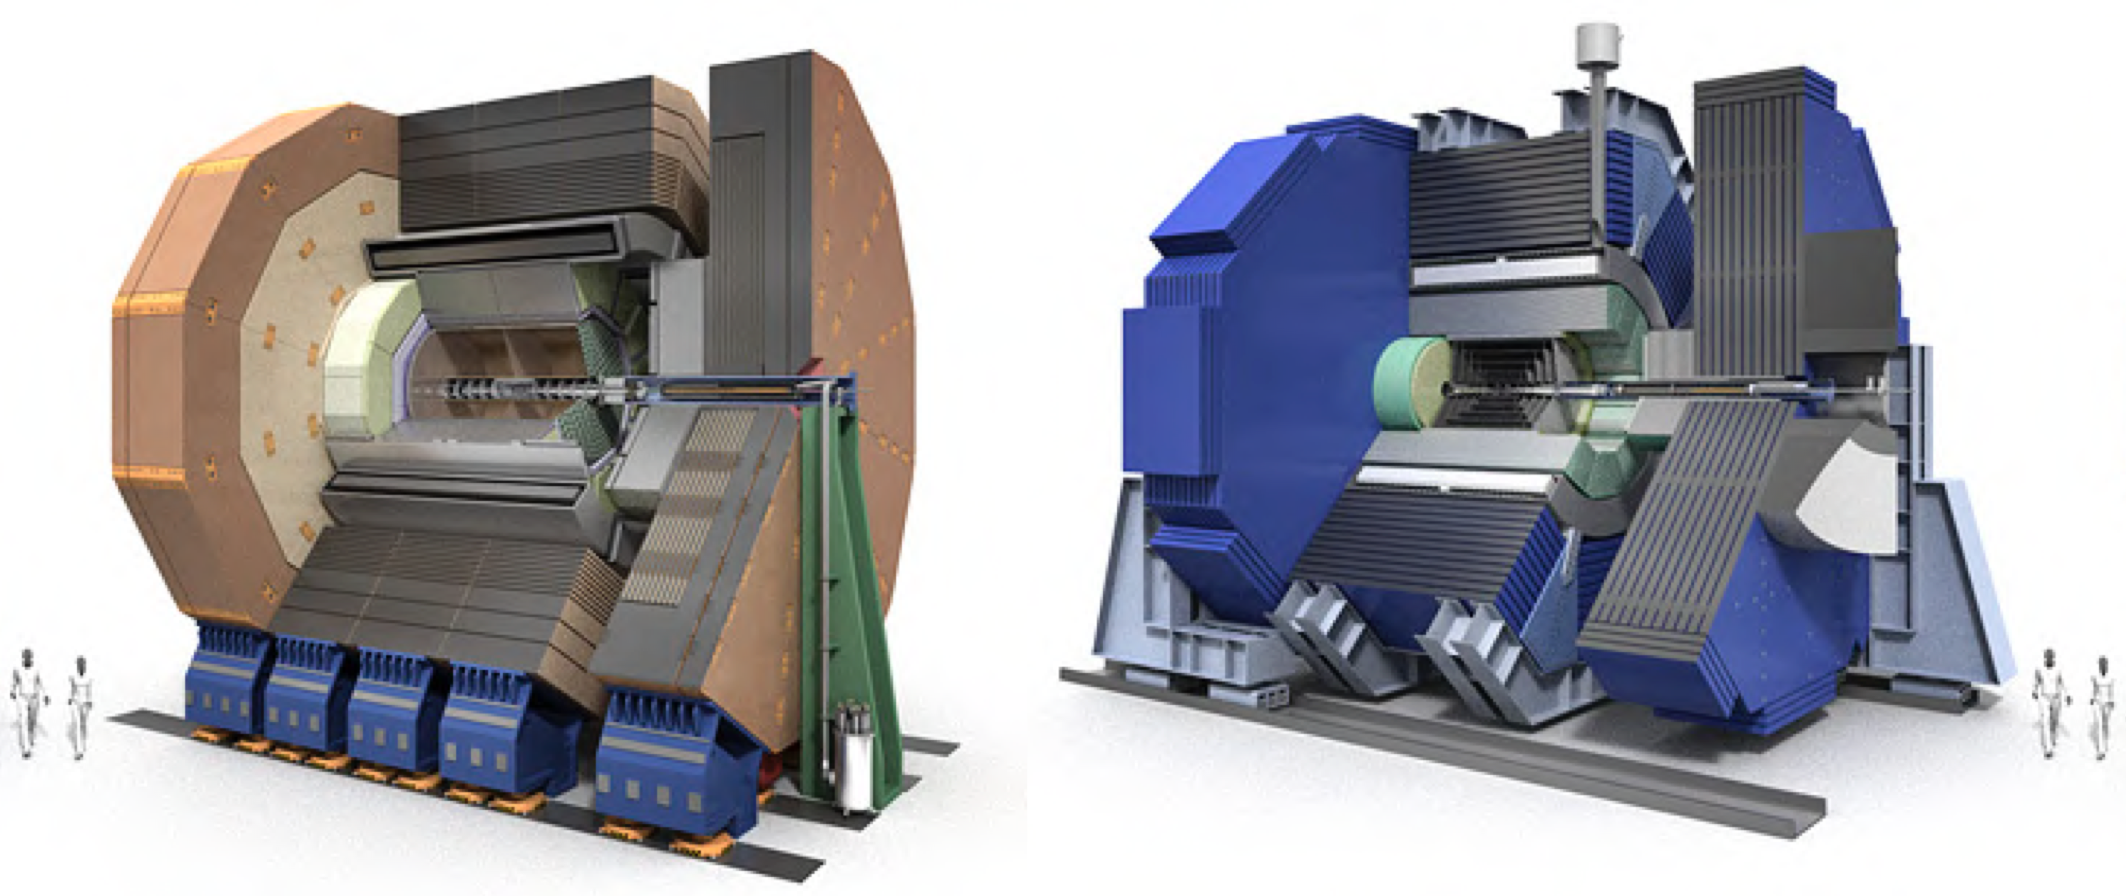
\includegraphics[keepaspectratio, scale=0.4]
 	{Figure/Introduction/detector.png}
 		\caption{(左) ILD (右) SiD の全体図}
 		\label{detector}
	\end{center}
\end{figure}
\subsection{International Large Detector: ILD}
ILD は内側から順に崩壊点検出器、飛跡検出器、電磁カロリメータ、ハドロンカロリメータ、ミューオン検出器で構成されている。カロリメータとミューオン検出器の間には3.5Tのソレノイドコイルが設置されている。図\ref{ild}に断面図を記す。
\begin{figure}[h]
	\begin{center}
 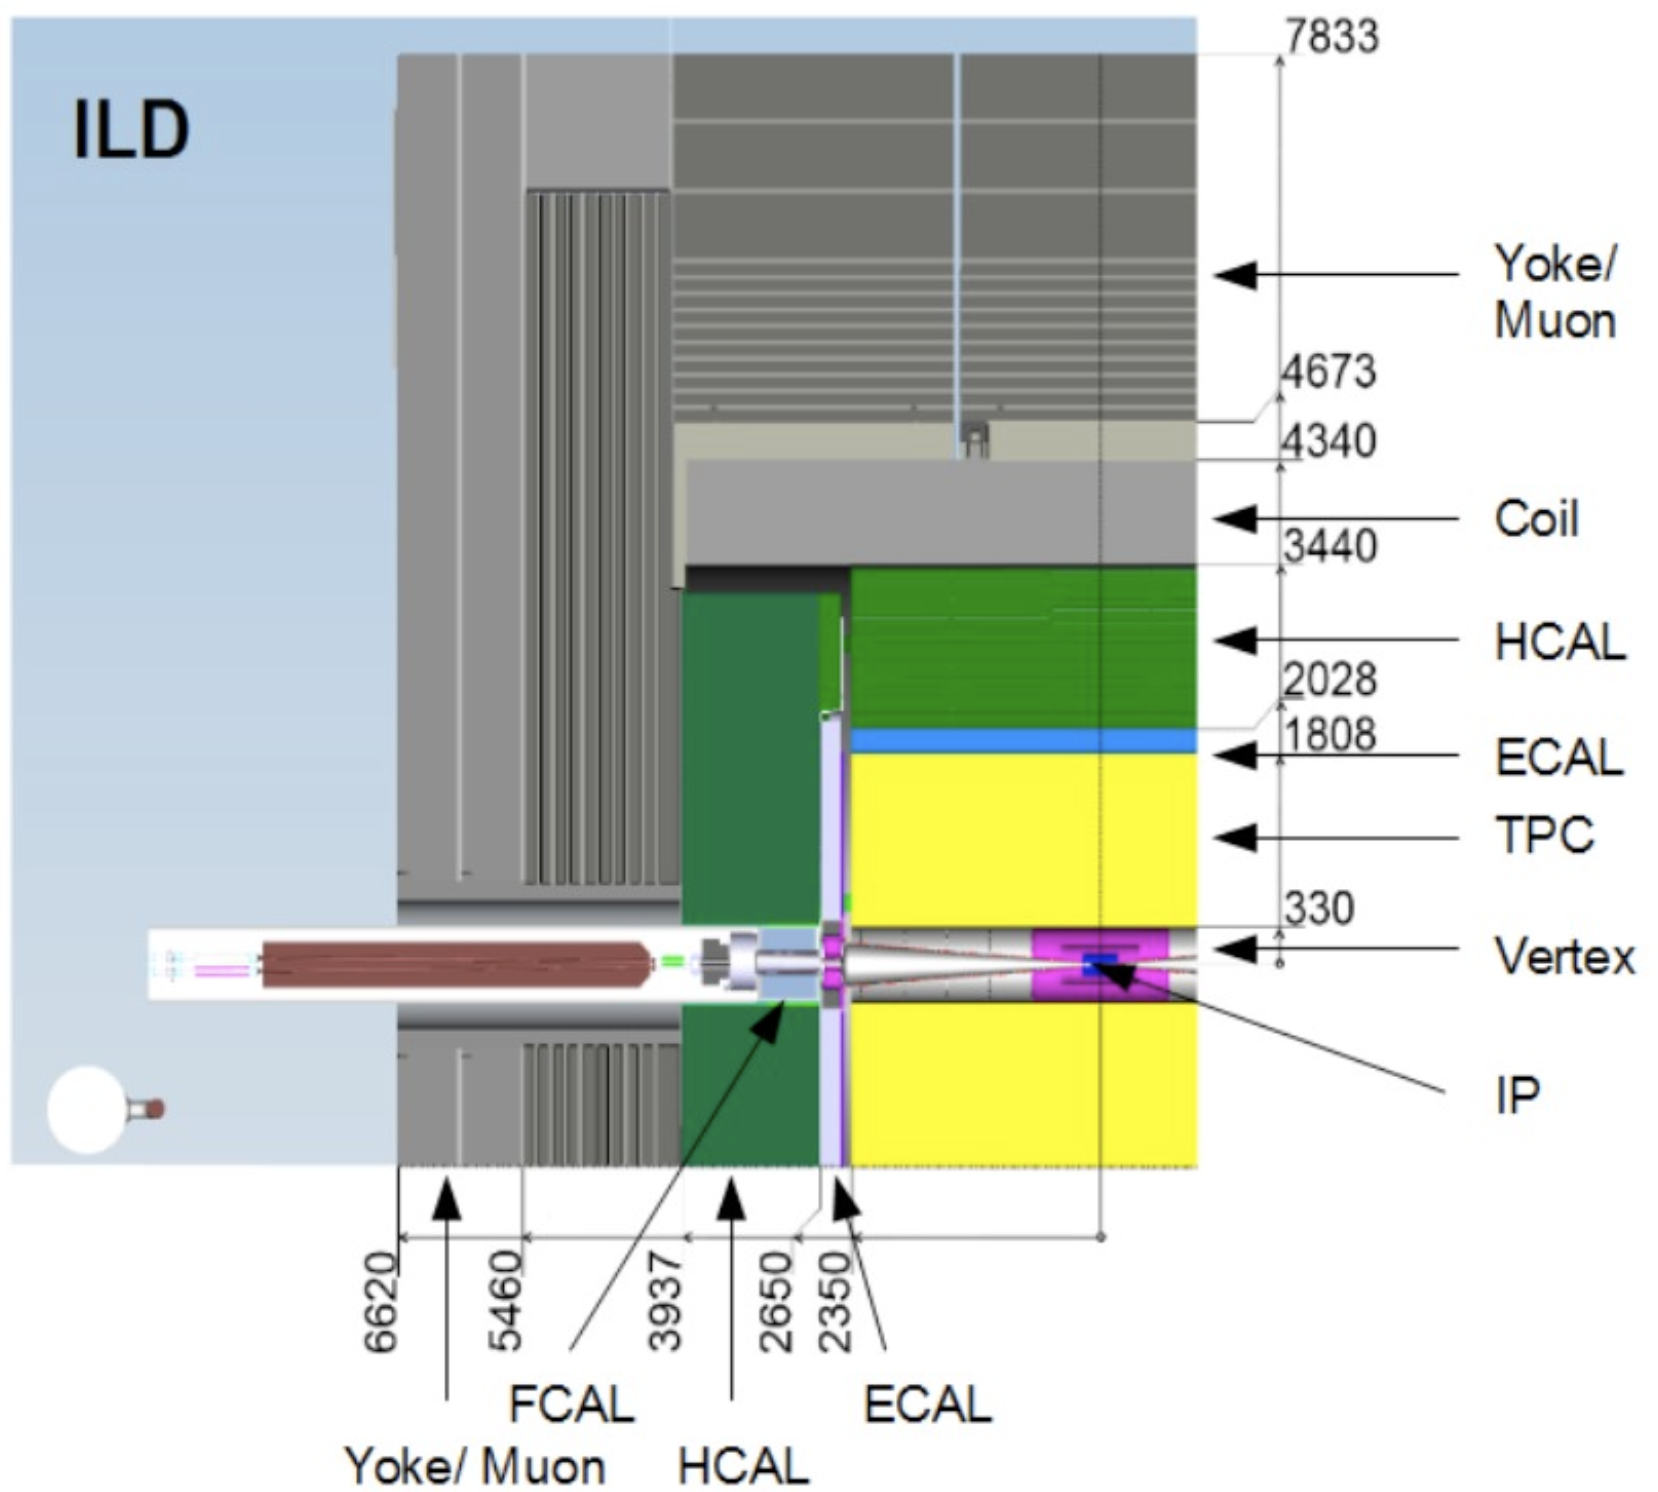
\includegraphics[keepaspectratio, scale=0.3]
 	{Figure/Introduction/ild.png}
 		\caption {ILDの断面図}
 		\label{ild}
	\end{center}
\end{figure}
\subsubsection{崩壊点検出器}
崩壊点検出器は、IPに最も近い場所に置かれる検出器であり、シリコンピクセルセンサーによって高い分解能で荷電粒子の生成点を測定する。飛跡の高精度な測定によって、短寿命粒子の崩壊点を高精度に再構成することができ、ILCでは小型化や高速読み出しに向けてCMOSセンサー、DEPFET、Fine Pitch CCD、SOIなど様々な技術候補が研究されている。
\subsubsection{中央飛跡検出器}
中央飛跡検出器は崩壊点検出器の外側に位置しており、Time Projection Chamber(TPC)とその周囲に設置されるシリコン検出器のハイブリッドで構成されている。TPCは大型のガスチェンバーであり、荷電粒子の通過でガス内に生じる電離電子を電極間にかけられた電場によってドリフトし、ドリフト時間などの情報をもとに飛跡を3次元的に再構成する検出器である。また荷電粒子の飛跡を再構成することで運動量の測定や、信号の大きさからエネルギー損失を測定することができ、粒子識別において重要な役割を果たす。
\subsubsection{カロリメータ}
カロリメータは入射粒子のエネルギーを測定するための検出器で、ILDでは内側から電磁カロリメータ(ECAL)、ハドロンカロリメータ(HCAL)によって構成されており、またビーム軸方向に対して前方カロリメータ(FCAL)が設置される。これらILDのカロリメータにはサンプリング型カロリメータが提案されており、シャワーを起こすための吸収層と生成されたシャワー内の粒子のエネルギーを測定する検出層が交互に組み合わさった構造となっている。\\
 電磁カロリメータは主に電磁シャワー内の光子のエネルギーを測定するために利用される。ILDでは後述のPFAのためジェット内の粒子を分離できる高精細なカロリメータが必要とされており、吸収層には物質量が大きいため放射長が短く、モリエール半径の小さいタングステンが検討されている。また、検出層には読み出しセルが高精細なシリコン検出器を用いるシリコン電磁カロリメータ(SiECAL)やシンチレータストリップを用いるシンチレータカロリメータ(ScECAL)が提案されている。\\
 ハドロンカロリメータは中性ハドロンのエネルギーを測定するための検出器である。HCALはECALに比べ大型であるため吸収層には鉄が用いられ、検出層には 3cm角のSiPMタイルを用いてシンチレーション光を検出するアナログカロリメータ(AHCAL)と、1cm角のセルをRPCを用いてバイナリ信号で読み出すデジタルカロリメータ(SDHCAL)の2つが提案されている。
\subsubsection{ミューオン検出器}
ミューオン検出器はその名の通りミューオンを検出する検出器である。ミューオンは他の検出器と相互作用を起こさないためIPから遠い検出器の最も外側に設置されており、RPCチェンバーとSiPMシンチレータストリップの両方が検討されている。

\section{ILCのソフトウェア}
\subsection{イベントジェネレータと検出器シミュレーション}
ILCをはじめとする線型加速器には「iLCSoft」というソフトウェアフレームワークが開発されており、検出器シミュレーションから事象再構成までを実行することができる。iLCSoft内では専用のLCIOフォーマットを使用し、C++アプリケーションフレームワークであるMarlinによって運用され、検出器のジオメトリなど検出器記述にはDD4hepというツールキットを使用するという点で統一されている。\\
 ILCは将来実験計画であるため、現在実験データは存在しないがシミュレーションによって検出器応答や新物理探索など研究が可能であり、本論文における研究で使用するデータもシミュレーションデータである。シミュレーションにおいてはまず、モンテカルロ(Monte Carlo, MC)法に基づくwizardというイベントジェネレータを用いて、標準理論や様々な理論を背景とした目的のイベントを背景信号とともに生成する。生成されたイベントに対してGeant4をベースとした検出器シミュレーションを実行し、粒子から検出器ヒットデータが生成される。
\subsection{事象再構成}
前節までで生成された検出器ヒットをもとに、粒子のエネルギーや飛跡を推定する事象再構成が行われる。
\subsubsection{Particle Flow Algorithm: PFA}
ILCの電子陽電子衝突で生じる粒子は、ジェットの終状態で検出される。このジェットのエネルギーは粒子識別や事象再構成において重要であり、ILCではジェットエネルギー分解能$\sigma_E/E=30\%/\sqrt{E(GeV)}$を目指している。これを達成するために導入されているアルゴリズムがParticle Flow Algorith(PFA)である。PFAはジェット内の粒子をその種類ごとに最適な検出器でエネルギー測定を行うことでジェットエネルギー分解能を向上させる手法であり、ジェット中に含まれる主な粒子の種類とそれに対応する検出器について表\ref{pfa}に示す。
\begin{table}[h]
 \centering
  \begin{tabular}{clll}
   \hline
   崩壊モード & \cth{崩壊分岐比} & \cth{ジェット内のエネルギー割合}\\
   \hline \hline
   荷電粒子 & \cth{飛跡検出器} &  \cth{62\%}\\
   光子 & \cth{ECAL} &  \cth{27\%}\\
   中性ハドロン & \cth{HCAL} &  \cth{10\%}\\
   ニュートリノ & \cth{-} &  \cth{1\%}\\
   \hline
  \end{tabular}
   \caption{ジェットを占める各粒子と対応する検出器}
   \label{pfa}
\end{table}
\subsubsection{飛跡再構成}
多数の飛跡を含むジェットは各検出器を通過するため、検出器ヒットをもとにフィッティングを行うことで飛跡は再構成することができる。特に崩壊点検出器では主に飛跡の方向情報を、中央飛跡検出器では運動量や時間情報を取得し、様々なパターン認識アルゴリズムを有するMarlinTrkによって再構成される。ここで再構成された飛跡をもとに、さらに高次な再構成が行われる。
\subsubsection{崩壊点検出}
ジェットはIPで生成された粒子が崩壊を繰り返し、多くの飛跡を残すことで再構成される。この粒子が崩壊する点を崩壊点(Vertex)と呼び、特にIPをprimary vertex、そこで生成された粒子の一次崩壊点をsecondary vertexと呼ぶ。崩壊点検出アルゴリズムでは、2本以上の飛跡の交点をフィッティングすることで再構成している。iLCSoftにおいては崩壊点検出からフレーバー識別までをLCFIPlusというフレームワークで実行することができる。
\subsection{ジェットクラスタリング}
ジェットクラスタリングでは、再構成された崩壊点をもとに全飛跡に対してクラスタリングを行う。
\subsection{フレーバー識別}
崩壊点の情報や飛跡の情報など20程度の物理量をもとに、多変量解析によってジェットの親粒子のフレーバー識別が行われる。LCFIPlusではROOTのTMVAパッケージを使用して、従来の機械学習手法であるBoosted Decision Trees(BDTs)を用いて識別が行われている。
\section{本研究の目的}
 本研究の目的は、電子陽電子ヒッグスファクトリーであるILCにおけるジェット測定技術の開発である。またその中でも、シリコンタングステン電磁カロリメータの開発・性能評価、フレーバー識別アルゴリズムの開発の2つのテーマで研究を行った。\\
 シリコンタングステン電磁カロリメータには